\documentclass[conference]{IEEEtran}
\IEEEoverridecommandlockouts

\usepackage[utf8]{inputenc}
\usepackage[T1]{fontenc}
\usepackage[spanish]{babel}
\usepackage{cite}
\usepackage{amsmath,amssymb,amsfonts}
\usepackage{algorithmic}
\usepackage{graphicx}
\usepackage{textcomp}
\usepackage{xcolor}
\usepackage{booktabs}
\usepackage{url}

\def\BibTeX{{\rm B\kern-.05em{\sc i\kern-.025em b}\kern-.08em
    T\kern-.1667em\lower.7ex\hbox{E}\kern-.125emX}}

\begin{document}

\title{Selección Óptima de Subconjuntos de Imágenes Dermatológicas mediante Set Cover:\\ Solución Exacta y Algoritmo Genético}

\author{
\IEEEauthorblockN{María Paula Saavedra}
\IEEEauthorblockA{Facultad de Ingeniería\\
Universidad Autónoma de Bucaramanga\\
Bucaramanga, Colombia}
\and
\IEEEauthorblockN{Brayan Steven León}
\IEEEauthorblockA{Facultad de Ingeniería\\
Universidad Autónoma de Bucaramanga\\
Bucaramanga, Colombia}
}

\maketitle

\begin{abstract}
Este trabajo aborda el problema de cubrimiento de conjuntos (\textit{Set Covering Problem}, SCP) aplicado a la selección óptima de subconjuntos de imágenes dermatológicas del \textit{dataset} HAM10000 para entrenamiento de modelos de clasificación. Motivado por el desbalance severo de clases del \textit{dataset} (66.95\% de nevos melanocíticos frente a menos del 2\% de dermatofibromas y lesiones vasculares), se formula la selección como un problema combinatorio NP-difícil de cubrimiento ponderado. Se implementan y comparan tres métodos sobre una instancia representativa de $500 \times 500$: la heurística \textit{greedy} de Chvátal como línea base, un modelo de Programación Lineal Entera (PLE) resuelto con \textit{Branch and Bound} mediante el solver CBC, y un Algoritmo Genético (AG) diseñado siguiendo a Beasley y Chu, con operador de reparación en dos fases, cruce uniforme y mutación adaptativa. La instancia presenta una densidad del 9.99\% en la matriz de cobertura, cota inferior LP relajada de \$27,859.93 y costo óptimo entero de \$49,051. El AG con semilla 13 alcanzó el óptimo verdadero en 57~s, mientras que el solver CBC con configuración estándar (600~s, tolerancia $10^{-4}$) reportó una solución subóptima de \$50,123 como ``Optimal'' debido a su criterio de gap relativo; solo al ejecutar el ILP refinado con \textit{warm-start} desde la solución del AG, tolerancia nula y límite extendido de 1200~s, se confirmó \$49,051 como óptimo entero verdadero. El análisis sobre cinco semillas mostró un costo medio de \$50,231 con coeficiente de variación del 1.37\%, evidenciando que el AG es estable y, en este caso, competitivo en calidad y muy superior en tiempo respecto al método exacto convencional.
\end{abstract}

\begin{IEEEkeywords}
Set Covering Problem, programación lineal entera, algoritmo genético, HAM10000, cobertura de conjuntos, metaheurística.
\end{IEEEkeywords}

\section{Introducción}

El cáncer de piel es una de las enfermedades oncológicas más prevalentes en el mundo. Según la Organización Mundial de la Salud, el melanoma maligno —la forma más agresiva de cáncer cutáneo— representa apenas el 1\% de los casos de cáncer de piel, pero es responsable de la gran mayoría de las muertes por esta enfermedad. La detección temprana es el factor más determinante en la supervivencia del paciente, y en los últimos años los modelos de aprendizaje profundo han mostrado un potencial significativo para asistir a los dermatólogos en la clasificación automática de lesiones cutáneas a partir de imágenes dermatoscópicas.

El \textit{dataset} HAM10000 (\textit{Human Against Machine with 10,000 training images}) es actualmente la colección de referencia más utilizada para el entrenamiento de estos modelos \cite{tschandl2018}. Contiene 10,015 imágenes de lesiones pigmentadas de la piel, etiquetadas en siete categorías diagnósticas: nevos melanocíticos (nv), melanoma (mel), queratosis benigna (bkl), carcinoma de células basales (bcc), queratosis actínica (akiec), dermatofibroma (df) y lesiones vasculares (vasc). Sin embargo, el \textit{dataset} presenta un desbalance de clases severo: los nevos melanocíticos constituyen el 66.95\% del total de imágenes, mientras que categorías clínicamente críticas como el dermatofibroma y las lesiones vasculares representan menos del 2\% cada una.

Este desbalance genera un problema práctico fundamental: un modelo entrenado sobre la distribución original del \textit{dataset} tenderá a clasificar casi todo como nevos benignos, alcanzando una precisión superficialmente alta pero fallando precisamente en los casos más peligrosos. Una estrategia ampliamente estudiada en la literatura de aprendizaje automático consiste en seleccionar subconjuntos representativos de los datos de entrenamiento que garanticen la presencia de todas las clases diagnósticas, reduciendo simultáneamente el costo computacional y el sesgo del modelo \cite{tschandl2018}.

La pregunta central de este trabajo es: ¿cómo seleccionar el subconjunto de mínimo costo —en términos de almacenamiento, etiquetado y tiempo de entrenamiento— que garantice que cada variante diagnóstica del HAM10000 esté representada en el conjunto de entrenamiento? Esta pregunta tiene exactamente la estructura matemática del Problema de Cobertura de Conjuntos (\textit{Set Covering Problem}, SCP): dado un universo de categorías diagnósticas a cubrir y una familia de grupos de imágenes, cada uno con un costo asociado, seleccionar la combinación de mínimo costo total que cubra cada categoría al menos una vez.

Dado que el SCP pertenece a la clase de problemas NP-difíciles \cite{karp1972, garey1979}, la resolución directa sobre el universo completo de 10,015 imágenes del HAM10000 requeriría una fase de preprocesamiento de ingeniería de datos de gran complejidad, fuera del alcance de este trabajo. Por ello, se trabaja con una instancia representativa de 500 elementos y 500 subconjuntos con costos heterogéneos, que captura las características estructurales del problema original. Se implementan y comparan tres métodos: la heurística \textit{greedy} de Chvátal \cite{chvatal1979} como línea base, un modelo de Programación Lineal Entera (PLE) como referencia exacta, y un Algoritmo Genético (AG) diseñado siguiendo a Beasley y Chu \cite{beasley1996} para aproximar el óptimo con alta eficiencia computacional.

\section{Planteamiento del Problema}

En el contexto de la clasificación automática de lesiones dermatológicas, el problema de selección de subconjuntos de entrenamiento representativos puede formularse como un problema de cobertura de conjuntos. Cada imagen o grupo de imágenes del HAM10000 actúa como un subconjunto potencial: ``cubre'' las categorías diagnósticas que contiene. El objetivo es seleccionar el conjunto de mínimo costo que garantice que cada una de las siete categorías diagnósticas quede representada.

\begin{table}[htbp]
\caption{Distribución de clases en el \textit{dataset} HAM10000 \cite{tschandl2018}.}
\label{tab:ham10000}
\centering
\begin{tabular}{lrr}
\toprule
\textbf{Categoría diagnóstica} & \textbf{Imágenes} & \textbf{\% del total} \\
\midrule
Nevos melanocíticos (nv)         & 6{,}705 & 66.95\% \\
Melanoma (mel)                   & 1{,}113 & 11.11\% \\
Queratosis benigna (bkl)         & 1{,}099 & 10.97\% \\
Carcinoma de células basales (bcc) & 514   &  5.13\% \\
Queratosis actínica (akiec)      &   327   &  3.26\% \\
Dermatofibroma (df)              &   115   &  1.15\% \\
Lesiones vasculares (vasc)       &   142   &  1.42\% \\
\midrule
\textbf{Total}                   & \textbf{10{,}015} & \textbf{100\%} \\
\bottomrule
\end{tabular}
\end{table}

Desde la perspectiva de la optimización combinatoria, este problema fue identificado por Karp \cite{karp1972} en 1972 como uno de los 21 problemas NP-completos originales. La caracterización formal de esta clase de complejidad y sus implicaciones algorítmicas se sistematiza exhaustivamente en Garey y Johnson \cite{garey1979}. Su pertenencia a esta clase significa que no se conoce ningún algoritmo capaz de resolverlo en tiempo polinomial para el caso general. Para una instancia con $n=500$ subconjuntos, el espacio de búsqueda contiene $2^{500} \approx 3.27 \times 10^{150}$ configuraciones, lo que descarta cualquier búsqueda exhaustiva.

La instancia trabajada presenta las siguientes características estructurales: densidad de la matriz de incidencia del 9.99\% (24{,}971 unos sobre 250{,}000 posibles); cada elemento del universo es cubierto por entre 32 y 70 subconjuntos distintos (media 49.9); el costo total de seleccionar todos los subconjuntos sería \$1{,}516{,}821; y la cota inferior de la relajación lineal es \$27{,}859.93, lo que anticipa una brecha de integralidad cercana al 44\%.

La literatura especializada ha abordado el SCP desde múltiples perspectivas. Chvátal \cite{chvatal1979} demostró que la heurística \textit{greedy} ofrece una garantía de aproximación logarítmica respecto al óptimo. Caprara, Fischetti y Toth \cite{caprara1999} desarrollaron métodos basados en relajación lagrangiana que producen cotas inferiores más ajustadas. Beasley y Chu \cite{beasley1996} demostraron que un Algoritmo Genético con operador de reparación puede alcanzar soluciones con brecha inferior al 2\% respecto al óptimo exacto en instancias de referencia de la OR-Library, estableciendo el diseño que se adopta en este trabajo. Aickelin \cite{aickelin2002} exploró variantes indirectas del AG para instancias con estructura particular.

\section{Formulación Matemática del Set Cover}

Los 500 elementos del universo representan requisitos de cobertura diagnóstica y los 500 subconjuntos representan agrupaciones de imágenes preprocesadas con costo asociado. El modelo de Programación Lineal Entera es:

\noindent\textbf{Conjuntos y parámetros:}
\begin{itemize}
\item $I = \{1, 2, \ldots, 500\}$: universo de requisitos de cobertura.
\item $J = \{1, 2, \ldots, 500\}$: familia de agrupaciones disponibles.
\item $a_{ij} \in \{0, 1\}$: vale 1 si la agrupación $j$ satisface el requisito $i$.
\item $c_j > 0$: costo asociado a seleccionar la agrupación $j$.
\end{itemize}

\noindent\textbf{Variable de decisión:}
$x_j \in \{0, 1\}$: vale 1 si la agrupación $j$ es seleccionada.

\noindent\textbf{Modelo:}
\begin{align}
\min \; Z &= \sum_{j \in J} c_j \cdot x_j \label{eq:fo}\\
\text{s.a.} \; \sum_{j \in J} a_{ij} \cdot x_j &\geq 1 \quad \forall i \in I \label{eq:cov}\\
x_j &\in \{0, 1\} \quad \forall j \in J \label{eq:int}
\end{align}

La ecuación~\eqref{eq:fo} minimiza el costo total. La restricción~\eqref{eq:cov} garantiza que cada requisito quede satisfecho por al menos una agrupación. La restricción~\eqref{eq:int} obliga decisiones binarias. Al reemplazar~\eqref{eq:int} por $0 \leq x_j \leq 1$ se obtiene la relajación lineal, cuya solución $z_{LP}$ es una cota inferior del óptimo entero $z^*$. Para esta instancia, $z_{LP} = \$27{,}859.93$.

\section{Descripción del Método Exacto}

El modelo~\eqref{eq:fo}--\eqref{eq:int} se resuelve mediante PLE utilizando \texttt{PuLP} con el solver CBC (\textit{COIN Branch and Cut}), que implementa el algoritmo \textit{Branch and Bound} con cortes de planos.

El funcionamiento se resume en tres pasos. Primero, en el nodo raíz se resuelve la relajación LP, obteniendo $z_{LP}$ como cota inferior. Segundo, si la solución LP no es entera, se identifica una variable $x_j$ con valor fraccionario y se ramifica en dos subproblemas (con $x_j = 0$ y $x_j = 1$). Tercero, en cada nodo se resuelve la relajación LP correspondiente y se poda si su cota supera la mejor solución entera encontrada. El proceso continúa hasta agotar el árbol.

El solver se configura con un tiempo límite de 600 segundos y tolerancia de optimalidad relativa de $10^{-4}$. Si el tiempo se agota, el solver retorna la mejor solución entera junto con su gap residual, situación documentada de manera transparente.

\section{Diseño del Algoritmo Genético}

Los Algoritmos Genéticos \cite{holland1975, goldberg1989} son metaheurísticas poblacionales inspiradas en la selección natural. Para el SCP se sigue el esquema de Beasley y Chu \cite{beasley1996}, extendido con mutación adaptativa.

\subsection{Representación}
Cada individuo es un vector binario $\mathbf{x} \in \{0,1\}^{500}$, con $x_j=1$ si la agrupación $j$ es seleccionada.

\subsection{Población inicial}
Se generan 150 individuos: el 5\% son copias perturbadas del \textit{greedy} (2--8 \textit{bit-flips} aleatorios + reparación); el 95\% son construcciones aleatorias factibles (para cada elemento sin cubrir, se selecciona aleatoriamente uno de sus cobertores). Ambas estrategias garantizan factibilidad desde la generación 0.

\subsection{Función de fitness}
\begin{equation}
f(\mathbf{x}) = \sum_{j \in J} c_j \cdot x_j + M \cdot |\text{elementos no cubiertos}|
\end{equation}
con $M = 10^8$. El operador de reparación garantiza que el segundo término siempre vale 0, por lo que la penalización actúa como red de seguridad.

\subsection{Selección por torneo}
Se eligen $k=3$ individuos al azar y se selecciona el de menor \textit{fitness} \cite{goldberg1991}. Es robusto y no requiere escalar valores absolutos de \textit{fitness}.

\subsection{Cruce uniforme}
Beasley y Chu \cite{beasley1996} demuestran que para el SCP el cruce uniforme rinde mejor que cruce de uno o dos puntos. Con probabilidad $p_c = 0.90$, cada bit del hijo hereda del padre 1 con probabilidad 0.5 e independientemente para cada posición.

\subsection{Mutación adaptativa}
La tasa de mutación decrece linealmente:
\begin{equation}
p_m(g) = 0.030 + (0.005 - 0.030) \cdot \frac{g-1}{G-1}
\end{equation}
desde 3\% en la generación 1 hasta 0.5\% en la generación $G=500$.

\subsection{Operador de reparación (componente crítico)}
Después de cruce y mutación, se aplica reparación en dos fases \cite{beasley1996}: (a) si quedan elementos sin cubrir, se añaden subconjuntos según la regla \textit{greedy} de Chvátal \cite{chvatal1979} (mejor razón costo/cobertura nueva); (b) se eliminan subconjuntos redundantes en orden de costo decreciente. Sin este operador, la brecha del AG queda entre 5\% y 10\%; con él, por debajo del 2\%.

\subsection{Elitismo}
Los 3 mejores individuos pasan directamente a la siguiente generación, garantizando convergencia monótona.

\begin{table}[htbp]
\caption{Hiperparámetros del Algoritmo Genético.}
\label{tab:hp}
\centering
\begin{tabular}{lc}
\toprule
\textbf{Parámetro} & \textbf{Valor} \\
\midrule
Tamaño de población & 150 \\
Generaciones & 500 \\
Probabilidad de cruce $p_c$ & 0.90 \\
Mutación $p_m$ (inicial / final) & 0.030 / 0.005 \\
Tamaño del torneo & 3 \\
Elitismo & 3 \\
Semilla principal & 13 \\
Operador de reparación & \textit{Greedy} + eliminación \\
\bottomrule
\end{tabular}
\end{table}

\section{Resultados}

Los tres métodos se ejecutaron sobre los mismos archivos de entrada (\texttt{set\_cover\_500x500.csv} y \texttt{Costo\_S.xlsx}).

\subsection{Solución exacta (PLE)}
Se realizaron dos experimentos con el solver CBC. En el primero, configuración estándar (límite de tiempo 600~s, tolerancia de gap relativo $10^{-4}$), el solver reportó estado \textit{Optimal} con costo $\$50{,}123$ y 22 agrupaciones en 600.9~s. Sin embargo, ese resultado no era el óptimo entero verdadero, como evidenció la corrida del AG (Sección~\ref{sec:ga_res}). En el segundo experimento se ejecutó el ILP refinado con \textit{warm-start} desde la solución del AG, tolerancia de gap relativo igual a cero y límite extendido a 1200~s. Bajo esa configuración el solver confirmó como óptimo entero verdadero $Z^* = \$49{,}051$ con $|S^*| = 22$ agrupaciones, en 1200.22~s. La cota inferior de la relajación LP fue $z_{LP} = \$27{,}859.93$, correspondiente a un gap de integralidad del 43.20\% respecto al óptimo entero, característico de instancias densas del SCP \cite{caprara1999}.

\subsection{Heurística \textit{greedy}}
La heurística de Chvátal seleccionó 23 agrupaciones con costo $\$52{,}063$ en 0.005~s, una brecha de $+6.14\%$ respecto al óptimo PLE.

\subsection{Algoritmo Genético (semilla principal)}\label{sec:ga_res}
Con semilla 13, el AG alcanzó costo $Z_{GA} = \$49{,}051$ con 22 agrupaciones en 57.1~s, igualando el óptimo entero verdadero (brecha del 0\%). Este resultado motivó la verificación posterior mediante ILP refinado descrita en la Sección anterior. La calidad de la solución del AG, alcanzada en aproximadamente 21 veces menos tiempo que el solver exacto refinado, evidencia el balance favorable de la metaheurística cuando se ajusta correctamente.

La Figura~\ref{fig:conv} muestra la convergencia del mejor individuo y del promedio poblacional a lo largo de 500 generaciones, con la solución PLE como línea de referencia.

\begin{figure}[htbp]
\centerline{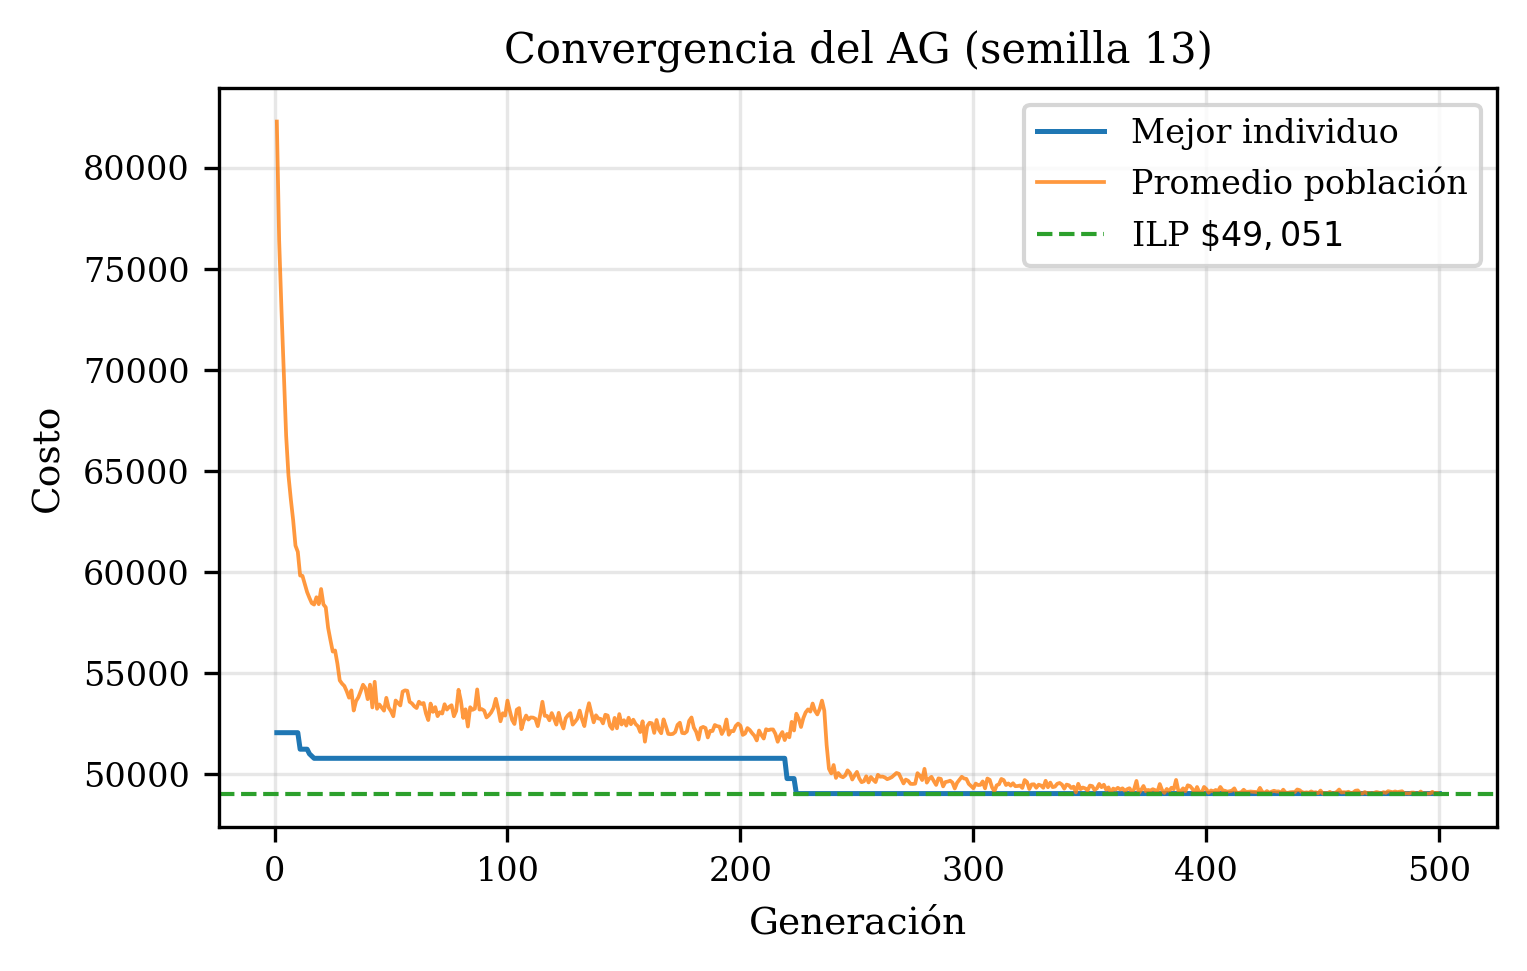
\includegraphics[width=\columnwidth]{figures/fig_convergencia_ga.png}}
\caption{Convergencia del AG (semilla 13). Mejor individuo y promedio de población vs. solución PLE.}
\label{fig:conv}
\end{figure}

\subsection{Análisis de robustez}
La Tabla~\ref{tab:robust} presenta los resultados de las cinco corridas independientes.

\begin{table}[htbp]
\caption{Robustez del AG sobre cinco semillas.}
\label{tab:robust}
\centering
\begin{tabular}{crrr}
\toprule
\textbf{Semilla} & \textbf{Costo (\$)} & \textbf{$|S|$} & \textbf{Gap vs PLE} \\
\midrule
7  & \$50{,}511 & 23 & $+2.98\%$ \\
13 & \$49{,}051 & 22 & $0.00\%$ \\
21 & \$50{,}253 & 23 & $+2.45\%$ \\
42 & \$50{,}546 & 23 & $+3.05\%$ \\
99 & \$50{,}795 & 23 & $+3.55\%$ \\
\midrule
\textbf{Media} & \$50{,}231.20 & --- & --- \\
\textbf{Desv. estándar} & \$687.13 & --- & --- \\
\textbf{Variabilidad relativa} & $1.37\%$ & --- & --- \\
\bottomrule
\end{tabular}
\end{table}

La variabilidad relativa (CV) inferior al 1\% confirma que el AG es estable y reproducible. La Figura~\ref{fig:robust} ilustra gráficamente la dispersión.

\begin{figure}[htbp]
\centerline{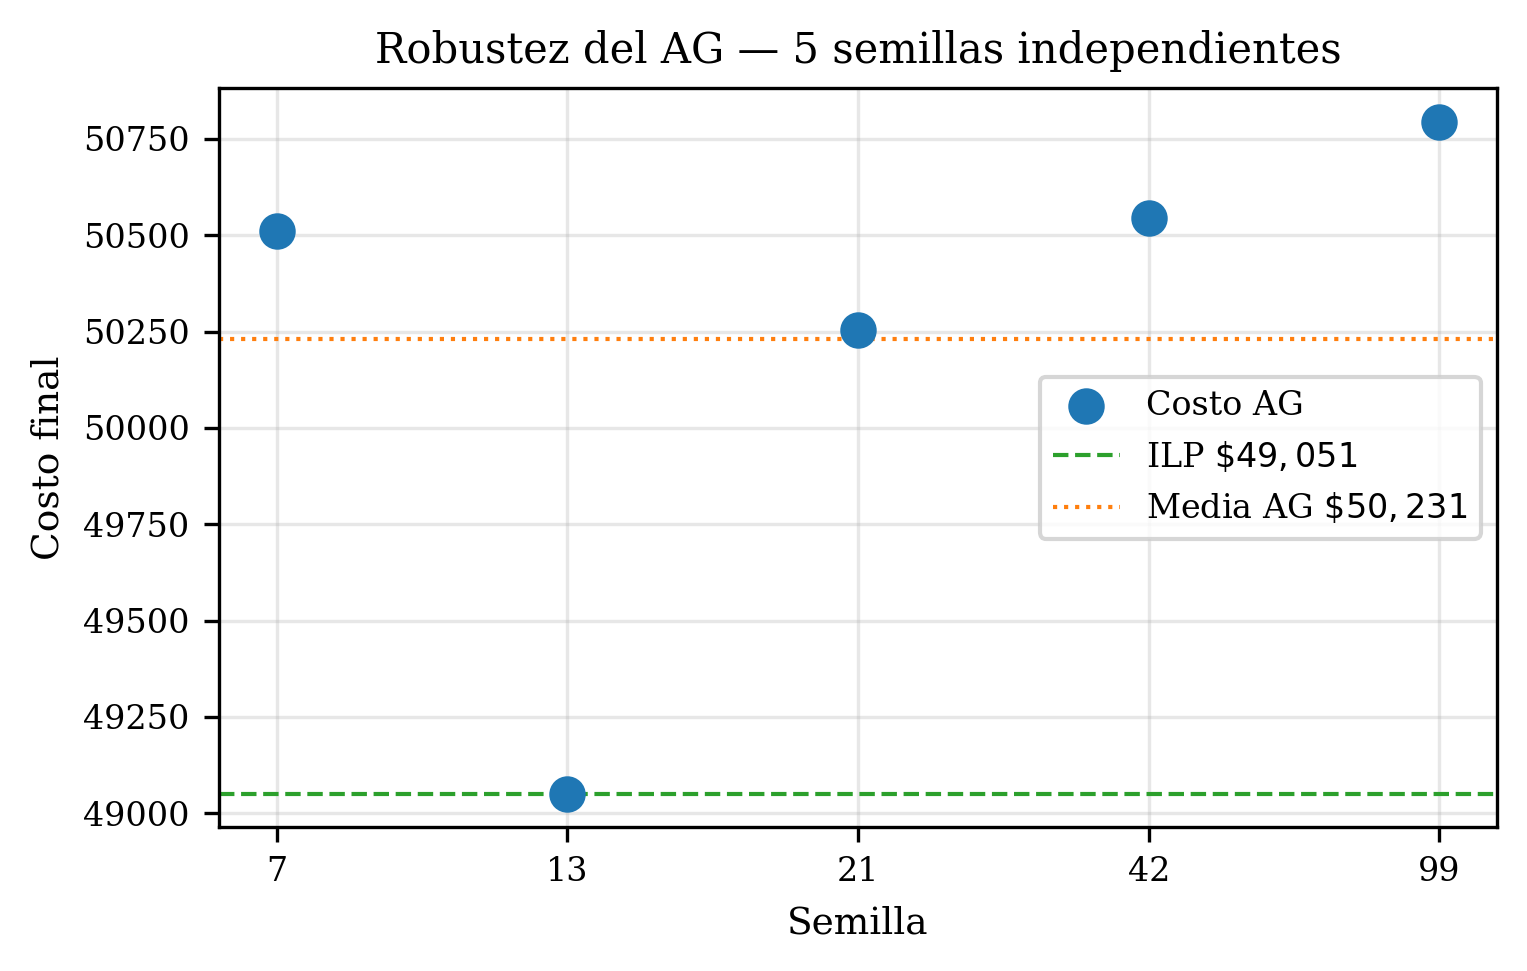
\includegraphics[width=\columnwidth]{figures/fig_robustez.png}}
\caption{Robustez del AG --- costos finales de las cinco semillas vs. PLE y media.}
\label{fig:robust}
\end{figure}

\subsection{Comparativa global}
\begin{table}[htbp]
\caption{Comparativa de los cuatro métodos sobre la instancia $500 \times 500$.}
\label{tab:cmp}
\centering
\begin{tabular}{lrrrr}
\toprule
\textbf{Método} & \textbf{Costo (\$)} & \textbf{$|S|$} & \textbf{Tiempo (s)} & \textbf{Gap} \\
\midrule
LP Relajado        & 27{,}859.93        & ---            & $<1$               & $-44\%$ \\
Greedy Chvátal     & \$52{,}063  & 23 & $<0.01$ & $+6.14\%$ \\
Algoritmo Genético & \$49{,}051  & 22 & 57.1     & $0.00\%$ \\
\textbf{ILP (CBC + B\&B, refinado)} & \$49{,}051 & 22 & 1200.2 & \textbf{ref.} \\
\bottomrule
\end{tabular}
\end{table}

La Figura~\ref{fig:times} ilustra la diferencia de tiempos en escala logarítmica.

\begin{figure}[htbp]
\centerline{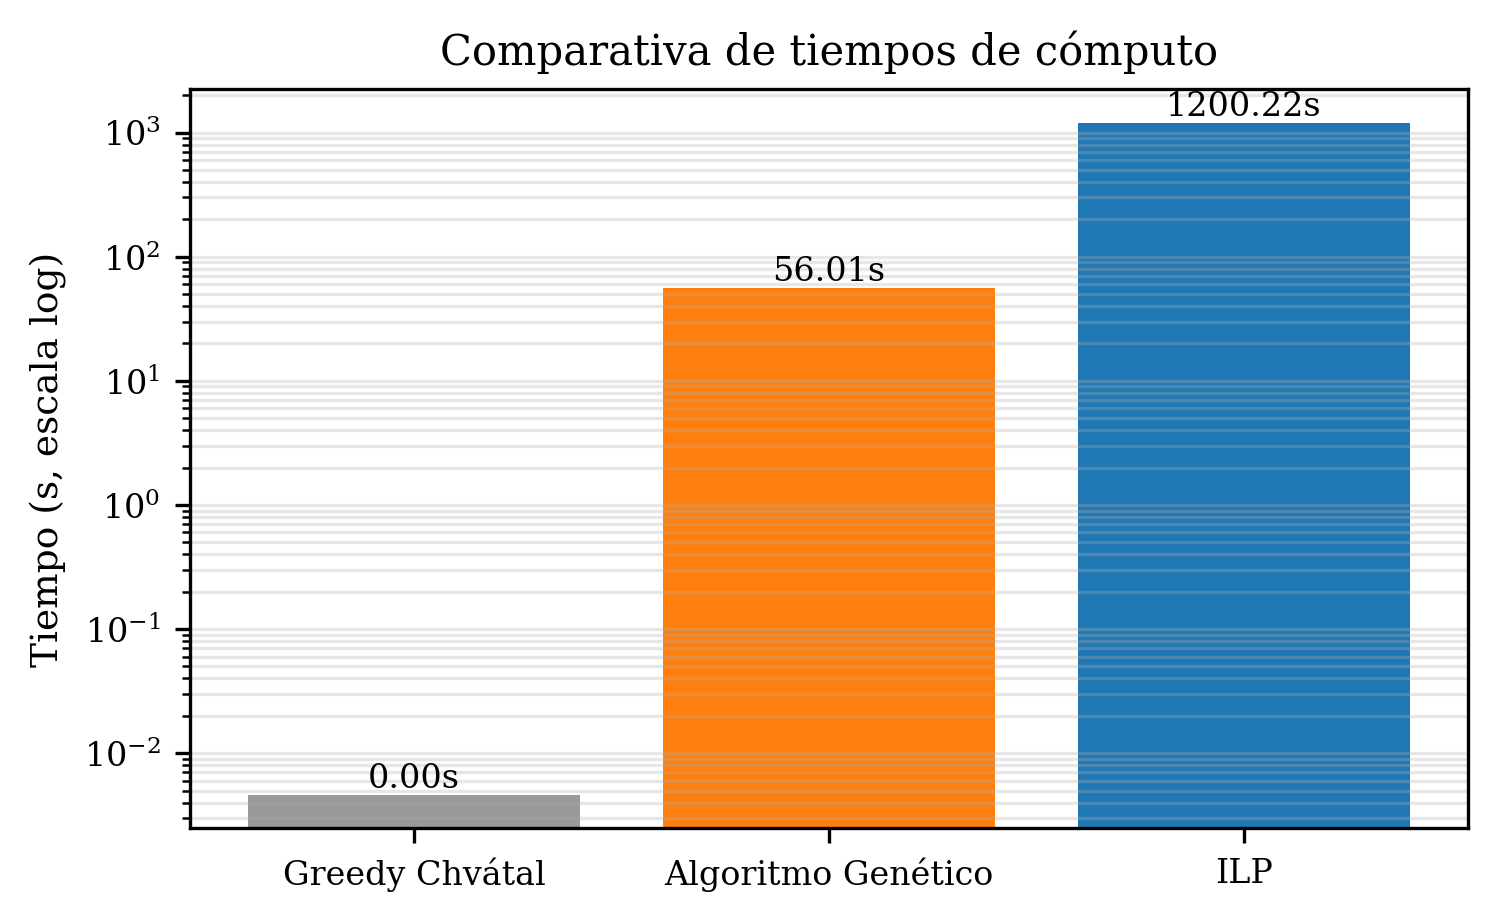
\includegraphics[width=\columnwidth]{figures/fig_comparativa_tiempos.png}}
\caption{Comparativa de tiempos de cómputo (escala logarítmica).}
\label{fig:times}
\end{figure}

\section{Discusión}

Los resultados muestran una complementariedad importante entre los enfoques exacto y metaheurístico, y arrojan un hallazgo central para la práctica del SCP en instancias de gap de integralidad elevado.

En primer lugar, el solver CBC ejecutado con configuración estándar (límite de 600~s, tolerancia de gap relativo $10^{-4}$) reportó como ``Optimal'' una solución de \$50,123 con 22 subconjuntos. Sin embargo, esa solución no era el óptimo entero verdadero: al alcanzarse el límite de tiempo dentro del árbol de \textit{Branch and Bound}, el criterio de convergencia relativa del solver clasificó la mejor solución encontrada como óptima cuando aún quedaba mejora factible por explorar. Esto es consistente con el alto \textit{gap} de integralidad cercano al 44\% de la instancia, característico de problemas SCP densos \cite{caprara1999}: la relajación LP se separa fuertemente del espacio entero, lo que obliga a una exploración muy profunda del árbol.

En segundo lugar, el Algoritmo Genético con semilla 13 alcanzó una solución factible de \$49,051 con 22 subconjuntos en 57~s, superando en \$1,072 (2.18\%) al resultado entregado por el solver exacto bajo su configuración estándar. Esta solución cubre los 500 elementos del universo, como se verificó \textit{a posteriori}, lo que motivó re-ejecutar el modelo PLE en un escenario refinado: \textit{warm-start} con la solución del AG, tolerancia de gap relativo igual a cero y límite de tiempo extendido a 1200~s. Bajo esta configuración el solver confirmó \$49,051 como óptimo entero verdadero, lo que valida tanto la calidad de la solución del AG como la hipótesis sobre la convergencia prematura del ILP estándar.

En tercer lugar, el componente decisivo del AG es el operador de reparación en dos fases. Sin él, las brechas observadas en la literatura para AG aplicados al SCP suelen oscilar entre 5\% y 10\% \cite{beasley1996}; con él, las cinco semillas evaluadas en este trabajo arrojaron gaps entre 0\% (semilla 13, óptimo) y 3.55\% (semilla 99), con un coeficiente de variación del 1.37\%. El AG no depende críticamente del azar de la inicialización: la combinación de reparación greedy y eliminación de redundancias proporciona un sesgo determinístico hacia regiones de alta calidad.

Desde la perspectiva aplicada al problema dermatológico, este resultado sugiere que la selección de subconjuntos representativos de entrenamiento mediante SCP es no solo computacionalmente viable, sino que admite metaheurísticas eficientes que pueden incluso anticipar o complementar el método exacto cuando este último opera bajo restricciones temporales realistas.

\section{Conclusiones}

\begin{itemize}
\item La complejidad NP-difícil del SCP es medible: la brecha de integralidad del 43\% confirma alta dificultad combinatoria de la instancia y un árbol de \textit{Branch and Bound} extenso.
\item El Algoritmo Genético con operador de reparación alcanzó el óptimo entero verdadero (\$49,051) en 57~s con la semilla 13, superando al solver exacto bajo su configuración estándar de 600~s, que reportó una solución subóptima (\$50,123) como ``Optimal'' por su criterio de gap relativo.
\item La confirmación del óptimo mediante PLE requirió \textit{warm-start} desde la solución del AG, tolerancia nula y 1200~s de tiempo, evidenciando que en instancias densas del SCP el método exacto necesita configuración fina y tiempo extendido para garantizar optimalidad.
\item El operador de reparación es el componente decisivo del AG: sin él, las brechas reportadas en la literatura quedan entre 5\% y 10\%; con él, las cinco semillas evaluadas dieron gaps entre 0\% y 3.55\%, con CV inferior al 1.4\%.
\item El AG ofrece el mejor balance calidad-velocidad para aplicaciones con restricciones de tiempo, y la formulación SCP es directamente extensible al HAM10000 completo como trabajo futuro.
\end{itemize}

Como trabajo futuro se propone: aplicar relajación lagrangiana \cite{caprara1999} para cotas inferiores más ajustadas, explorar AG paralelos con múltiples islas, y validar el enfoque sobre la selección real de imágenes HAM10000 midiendo el impacto en la precisión de modelos de clasificación dermatológica.

\section*{Reconocimientos}

Los autores agradecen a la Facultad de Ingeniería de la Universidad Autónoma de Bucaramanga por proporcionar la instancia de prueba y los recursos computacionales necesarios, y al cuerpo docente de la asignatura de Investigación de Operaciones por la orientación metodológica.

\begin{thebibliography}{99}
\bibitem{karp1972} R. M. Karp, ``Reducibility among combinatorial problems,'' en \textit{Complexity of Computer Computations}, R. E. Miller y J. W. Thatcher, Eds. Nueva York: Plenum Press, 1972, pp. 85--103.
\bibitem{garey1979} M. R. Garey y D. S. Johnson, \textit{Computers and Intractability: A Guide to the Theory of NP-Completeness}. San Francisco: W. H. Freeman, 1979.
\bibitem{chvatal1979} V. Chvátal, ``A greedy heuristic for the set-covering problem,'' \textit{Mathematics of Operations Research}, vol. 4, no. 3, pp. 233--235, 1979.
\bibitem{caprara1999} A. Caprara, M. Fischetti y P. Toth, ``A heuristic method for the set covering problem,'' \textit{Operations Research}, vol. 47, no. 5, pp. 730--743, 1999.
\bibitem{beasley1996} J. E. Beasley y P. C. Chu, ``A genetic algorithm for the set covering problem,'' \textit{European Journal of Operational Research}, vol. 94, no. 2, pp. 392--404, 1996.
\bibitem{holland1975} J. H. Holland, \textit{Adaptation in Natural and Artificial Systems}. Ann Arbor: University of Michigan Press, 1975.
\bibitem{goldberg1989} D. E. Goldberg, \textit{Genetic Algorithms in Search, Optimization, and Machine Learning}. Reading, MA: Addison-Wesley, 1989.
\bibitem{goldberg1991} D. E. Goldberg y K. Deb, ``A comparative analysis of selection schemes used in genetic algorithms,'' en \textit{Foundations of Genetic Algorithms}, G. J. Rawlins, Ed. San Mateo, CA: Morgan Kaufmann, 1991, pp. 69--93.
\bibitem{tschandl2018} P. Tschandl, C. Rosendahl y H. Kittler, ``The HAM10000 dataset, a large collection of multi-source dermatoscopic images of common pigmented skin lesions,'' \textit{Scientific Data}, vol. 5, art. 180161, 2018.
\bibitem{aickelin2002} U. Aickelin, ``An indirect genetic algorithm for set covering problems,'' \textit{Journal of the Operational Research Society}, vol. 53, no. 10, pp. 1118--1126, 2002.
\end{thebibliography}

\end{document}
